\subsection{Final Controller Design}
To be able to choose appropriate feedback and observer matrices, a simulation of the non linear system, including the network, is used. Different selections of gains are compared and their stability within the network is check to give the final design of the controller.

\autoref{}, \ref{}, \ref{} and \ref{} show the behavior of the system when using different approaches of choosing $Q_x$ and $Q_u$ matrices to design the state feedback matrix.

\begin{minipage}{\linewidth}
    \begin{minipage}{0.6\linewidth}
        \begin{figure}[H]
            \includegraphics[scale=.35]{figures/}
            \centering			
            \captionof{figure}{.}
            \label{attitudeController1}
        \end{figure}
    \end{minipage}
    \hspace{0.03\linewidth}
    \begin{minipage}{0.4\linewidth}
        \begin{figure}[H]\vspace{20mm}
            \includegraphics[scale=.35]{figures/}
            \centering \vspace{7mm}
            \captionof{figure}{.}
            \label{attitudeController2}
        \end{figure}
    \end{minipage}
\end{minipage}
\begin{minipage}{\linewidth}
    \begin{minipage}{0.5\linewidth}
        \begin{figure}[H]
            \includegraphics[scale=.35]{figures/}
            \centering			
            \captionof{figure}{.}
            \label{attitudeController3}
        \end{figure}
    \end{minipage}
    \hspace{0.03\linewidth}
    \begin{minipage}{0.5\linewidth}
        \begin{figure}[H]
            \includegraphics[scale=.35]{figures/}
            \centering
            \captionof{figure}{.}
            \label{attitudeController4}
        \end{figure}
    \end{minipage}
\end{minipage}

The design of the observer has also some influence in the final result, as too fast dynamics in the estimation can lead to an unstable observer. This can be seen in \autoref{} where a lot of oscillations are added and the  \fxnote{In the observer explanation maybe remove that we can choose the gain as high as we want}.
%
\begin{minipage}{\linewidth}
    \begin{minipage}{0.5\linewidth}
        \begin{figure}[H]
            \includegraphics[scale=.35]{figures/}
            \centering			
            \captionof{figure}{.}
            \label{attitudeControllerObserver1}
        \end{figure}
    \end{minipage}
    \hspace{0.03\linewidth}
    \begin{minipage}{0.5\linewidth}
        \begin{figure}[H]
            \includegraphics[scale=.35]{figures/}
            \centering
            \captionof{figure}{.}
            \label{attitudeControllerObserver2}
        \end{figure}
    \end{minipage}
\end{minipage}

The final design can be seen in \autoref{}, where a compromise between overshoot, fast response when returning to equilibrium and control action is chosen as the best approach.
        
\begin{minipage}{\linewidth}
    \begin{minipage}{0.5\linewidth}
        \begin{figure}[H]
            \includegraphics[scale=.35]{figures/}
            \centering			
            \captionof{figure}{.}
            \label{attitudeControllerFinal}
        \end{figure}
    \end{minipage}
    \hspace{0.03\linewidth}
    \begin{minipage}{0.5\linewidth}
        \begin{figure}[H]
            \includegraphics[scale=.35]{figures/}
            \centering
            \captionof{figure}{.}
            \label{attitudeControllerObserver}
        \end{figure}
    \end{minipage}
\end{minipage}

\begin{figure}[H]
    \includegraphics[scale=.35]{figures/}
    \centering			
    \captionof{figure}{.}
    \label{attitudeControllerAction}
\end{figure}
























%The performance of the attitude controller is evaluated by simulating it in the non-linear model. The simulation with the linearized model is not shown due to being almost identical to that of the non-linear model. \autoref{fig:AttitudeController} and \ref{fig:AttitudeControllerOutput} show the performed simulations.
%\begin{figure}[H]
%	\centering
%	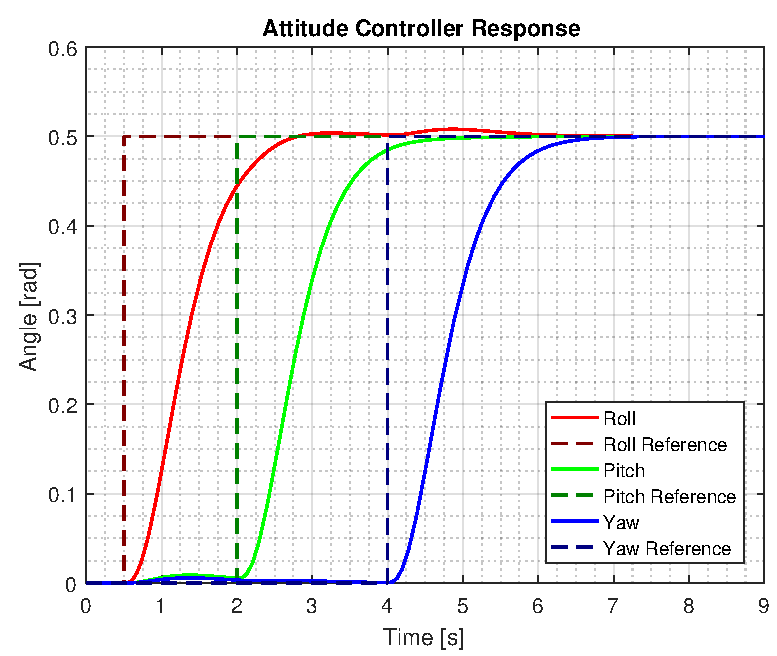
\includegraphics[scale=0.75]{figures/simAttitudeControl}
%	\caption{Step response of the attitude controller.}
%	\label{fig:AttitudeController}
%\end{figure}
%It can be seen that the controller reaches the given reference in approximately 2 seconds for the three angles. The coupled charateristic of the system is also present in the graphs as small bumps in two of the angles when the third angle is changed. The controller is capable of handling this situation.
%
%The control action required to achieve the previously seen response is shown in below. 
%\begin{figure}[H]
%	\centering
%	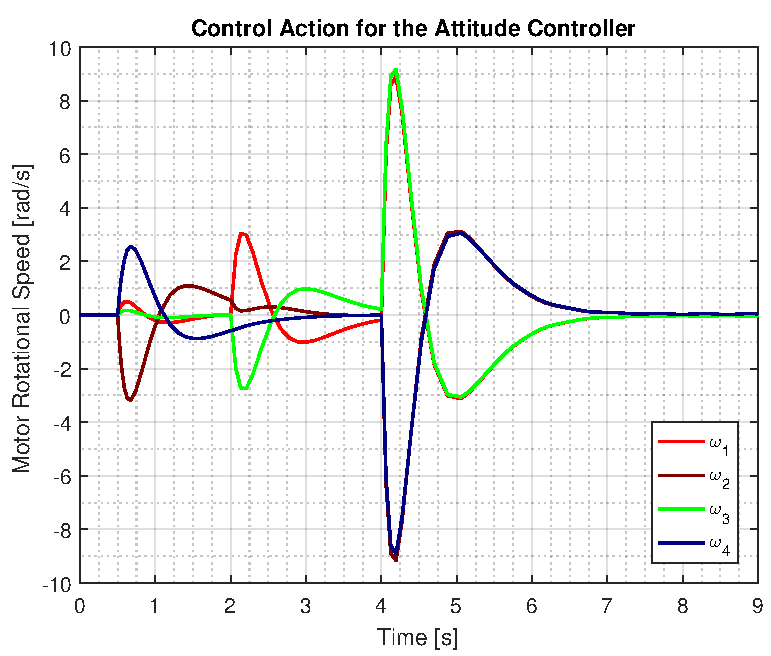
\includegraphics[scale=0.75]{figures/simAttitudeControlOutput}
%	\caption{Control output of the attitude controller, that is, the four motor rotational speeds.}
%	\label{fig:AttitudeControllerOutput}
%\end{figure}
%The required motor rotational speeds are represented as variations from the equilibrium rotational speeds of the motors. It can be seen that motors 1 and 3 change their speed when the roll angle is to be changed and motors 2 and 4 do the same for the pitch angle. In these cases, the maximum variation from equilibrium is approximately 3 rad/s. When the yaw angle is to be changed, the four rotational speeds are involved, requiring a peak variation of approximately 9 rad/s. 